% !TEX TS-program = pdflatex
% !TEX encoding = UTF-8 Unicode

% This is a simple template for a LaTeX document using the "article" class.
% See "book", "report", "letter" for other types of document.

\documentclass[11pt]{article} % use larger type; default would be 10pt

\usepackage[utf8]{inputenc} % set input encoding (not needed with XeLaTeX)

%%% Examples of Article customizations
% These packages are optional, depending whether you want the features they provide.
% See the LaTeX Companion or other references for full information.

%%% PAGE DIMENSIONS
\usepackage{geometry} % to change the page dimensions
\geometry{a4paper} % or letterpaper (US) or a5paper or....
% \geometry{margin=2in} % for example, change the margins to 2 inches all round
% \geometry{landscape} % set up the page for landscape
%   read geometry.pdf for detailed page layout information

\usepackage{graphicx} % support the \includegraphics command and options

% \usepackage[parfill]{parskip} % Activate to begin paragraphs with an empty line rather than an indent

%%% PACKAGES
\usepackage{booktabs} % for much better looking tables
\usepackage{array} % for better arrays (eg matrices) in maths
\usepackage{paralist} % very flexible & customisable lists (eg. enumerate/itemize, etc.)
\usepackage{verbatim} % adds environment for commenting out blocks of text & for better verbatim
\usepackage{subfig} % make it possible to include more than one captioned figure/table in a single float
% These packages are all incorporated in the memoir class to one degree or another...

%%% HEADERS & FOOTERS
\usepackage{fancyhdr} % This should be set AFTER setting up the page geometry
\pagestyle{fancy} % options: empty , plain , fancy
\renewcommand{\headrulewidth}{0pt} % customise the layout...
\lhead{}\chead{}\rhead{}
\lfoot{}\cfoot{\thepage}\rfoot{}

%%% SECTION TITLE APPEARANCE
\usepackage{sectsty}
\allsectionsfont{\sffamily\mdseries\upshape} % (See the fntguide.pdf for font help)
% (This matches ConTeXt defaults)

%%% ToC (table of contents) APPEARANCE
\usepackage[nottoc,notlof,notlot]{tocbibind} % Put the bibliography in the ToC
\usepackage[titles,subfigure]{tocloft} % Alter the style of the Table of Contents
\renewcommand{\cftsecfont}{\rmfamily\mdseries\upshape}
\renewcommand{\cftsecpagefont}{\rmfamily\mdseries\upshape} % No bold!

%%% END Article customizations

%%% The "real" document content comes below...

\title{Modélisation distribuée d’un jeu stratégique : 
 \\ Cas d'une variante du jeu de dames}
\author{CHUPIN Pierre-Henri \\ SOLOMON Maria}
\date{} % Activate to display a given date or no date (if empty),
         % otherwise the current date is printed 

\begin{document}
\maketitle

\begin{abstract}
Ce  projet  a  pour  but  de  créer  une modélisation distribuée et de l'appliquer à un cas concré ici une variente du jeu de dames. Nous avons fait en sorte de rendre chaque agent (pièce) indépendante dans leurs raisonnement et ils doivent communiquer entre eux afin de réussir à avoir les meilleurs résultat. Cela permettra de créer des stratégies pour des jeux et de comprendre mieux comment fonctionne la modélisation distribuée. Nous faisons un match entre deux IA qui utilise la même stratégie afin de voir les résultats avec deux joueurs au même niveau de compétance. \\
Mots-clés: Modélisation distribuée, stratégie, recherche de risque
\end{abstract}
\section{Introduction}
Ce projet s'inscrit dans le cadre du second semestre de Master 1 informatique de Lyon et dans l'optique de poursuivre en Master IA de Lyon. Pour ce projet nous avons put compter sur notre encadrant Aknine Samir appartenant à l'équipe Systèmes Multi-Agents de lyon. Depuis longtemps beaucoup d'informaticiens veulent résoudre des jeux comme les échecs en créant des IA cable de faire cela. Résoudre ce genre de problèmes demandes beaucoup de travail car il faut dans un premier temps créer informatiquement le jeux que l’on veut créer et mettre en place toutes ses règles. Une fois tout cela fait le vrai travail commence, le codage des stratégies que l’IA utilisera pour jouer au jeux. Nous avons décidé de faire la modélisation distribuée d'un jeu ancestrale, le jeu de dames. 

\section{Etat de l'art}

\subsection{Modélisation Distribuée}

\section{Outils utilisés}

\subsection{Le Jeu de dames}
La modélisation réalisé se base sur le jeux de dames classique mais avec quelque changement de régle qui permette d'avoir des comportements différents de ce qu'on peut voir en général. voici la liste des différentes régles et système utilisé utilisée:
\begin{itemize}
\item Un plateau carré de 10 cases sur 10
\item 20 pions blancs pour un joueur et 20 pions noir pour un autre joueur
\item chaque joueur jouera à tour de rôle et il pourra jouer 1 à N (nombre choisi avant de lancer une partie) pièces en même temps ce qui permet de voir comment vont réagir plusieurs pièces ensemble
\item Création classique de la dames qui permet d'avoir plusieurs types de pièce à gérer
\item Une dame peut se déplacer sur 3 cases de diagonale maximum nous avons voulu changer avec les règles habituels
\item La prise est obligatoire comme dans les règles classique des dames.
\item La prise multiple est possible aussi comme dans les dames classiques
\item Une partie est gagné si on prend toutes les pièces advairse ou si l'aderversaire ne peut pas ce déplacer quand c'est son tour de jeu.
\item Si il y a 30 coups sans prise la partie est nul
\end{itemize}

\section{Travail réalisé}

\subsection{Modélisation du jeu de dame}
Afin de commencé notre travail sur la modélisation distribuée nous avons du bien sur faire la modélisation du jeu de dame. Le fait de donner un aspect graphique au jeu ( on voit le plateau et les pièces ce déplacer) était important afin de mieux voir ce qu'il ce passe pendant le déroulement du programme et donner un coté graphique à notre travail. Bien sur on aurait pu le faire tourner sans affichage pour juste avoir le résultat de la simulation. Il a donc fallut partir à la recherche d'image pouvant être intégrer au projet qui permettrait de rendre cela possible. il nous fallait alors
\begin{itemize}
\item Une image de plateau carré de 10 cases sur 10
\item Une image de pion blanc et noir
\item Une image de dema blanche et noir
\end{itemize}
Une fois cela fait il nous suffit de mettre en place le plateau avec nos différentes images \cite{annexe1}. Voici donc à quoi ressemble le plateau et les pièces après le premier coup des blancs.

\begin{center}
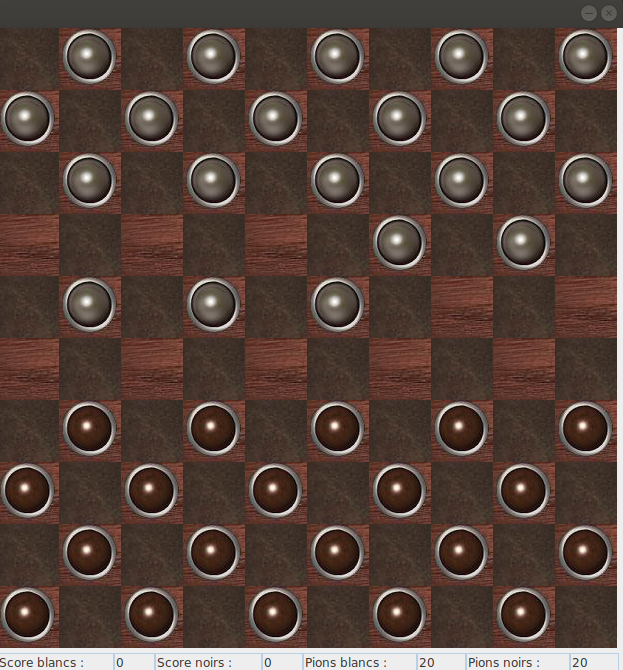
\includegraphics[scale=0.4]{plateau-ini}
\end{center}

afin de mieux pouvoir voir ce qu'il ce passe il a fallut mettre en place la possibilité de mettre en pause le jeu\cite{annexe2} pour s'arreter et comprendre au mieux comment le programme fonctionne, nous verrons par la suite des exemples précis de comportement. \\

\subsection{Stratégie Naive}
Avant de pouvoir commencer à aller loin dans la modélisation distribuée nous avons du faire une stratégie naive qui consiste simplement à faire jouer l'IA le plus simplement possible sans aucune réflexion de sa part. Nous sommes partie sur le principe que l'IA jouera le maximum de pions possible pour chaque coups. Dans un premier temps elle regardera les coups obligatoires à faire comme la prise et jouera toute les prises, si il lui reste des mouvements possible elle devra alors regarder chaque pièce non déplacé si elle peut les déplacer. Si oui alors elle la joue qu'importe si le mouvement est mauvais ou non jusqu'à ne plus avoir de mouvement possible à jouer. cette stratégie naive nous servira de base pour créer une stratégie plus performante par la suite.

\subsection{Amélioration de la prise}


\subsection{Amélioration du déplacement}
Il y avait comme soucis majeur le choix des pièces à déplacer une fois les coups obligatoires joué. Nous avons donc du réfléchir à comment faire pour éviter les mouvements mauvais (qui nous font perdre des pièces juste après). Pour ce faire nous avons cherché des algorithmes connu qui sont utilisé pour ce genre de problème. C'est le cas de l'algorithme min-max qui nous a inspiré. Le but est de tester à chaque fois qu'on prévoit de déplacer une pièce si cela est risqué pour elle ou non. Pour ce faire nous avons eu besoin de créer une fonction récursive qui test si la pièce que l'on veut jouer sera en danger si on l'a joue. Cela fait partie de la première étape de la fonction car le but de l'algorithme min-max est de fabriquer un arbre de toutes les possibilitées possible de mouvement et de déscendre le plus possible en profondeur. Le problème entant que l'arbre devient extrémement grand très rapidement. Exemple si on peut déplacer 10 pièce différentes et chacune à deux position différentes on aura un arbre degrès 20 sur le noeud racine mais cela ne s'arrete pas la car si on veut déscendre d'un cran et voir le déplacement que l'adversaire pourrait faire en réponse alors on a pour chaque neud touts les mouvements possible de l'adversaire et rappelon que nous donné la possibilité de déplacer au choix 1 à N pièce par coups ce qui augmente le nombre de déplacement adversaire possible et donc augmente la taille de l'arbre. C'est pour cet raison que nous avons voulu limité notre parcoure en profondeur de l'arbre et la façon dont nous cherchons dans l'arbre. au lieu de simuler tous l'arbre puis de chercher dedans nous le simulon petit à petit et nous arrêtons des que l'ont a trouvé un mouvement satisfaisant. Pour ce faire nous prenons les pièces une à une et quand elle peut ce déplacer alors nous testons si après avoir fait ce déplacement elle risque de se faire prendre par l'adversaire et si c'est le cas alors nous la jouons pas. au contraire si elle peut ce déplacer sans risque alors elle est joué et nous arretons de vérifier des que nous avons joué le nombre maximum de pièce possible dans notre coup ce qui fait que nous créons que petit à petit l'abre des coups possible afin de limiter la taille de celui ci. Bien sur cela implique des limites car certaines fois un coups sans risque par rapport à un autre est plus efficace.

\subsection{Amélioration du pistage du risque}
Nous avons vite remarquer des problèmes avec notre algorithme et surtout 1 majeur qui est que déplacer une pièce sans risque peut créer des risques sur une autre pièces ailleurs sur le plateau et cela n'est pas acceptable pour avoir une stratégie performante. Nous avons donc du réfléchir à comment faire pour éviter cela. Pour ce faire il a fallut faire communiquer toutes les pièces d'un même camps entre elle afin de tester si jouer un coup en particulier rendait une pièce sensible à la prise adversaire. Il a fallut alors tester toute les pièces pour chaque tantative de déplacement et à chaque fois aller plus loin qu'un seul coup. On voit ici encore mieux le problème de complexité qui peut très vite explosé si on essaye d'aller encore plus en profondeur. En plus de ce problème un autre important était à corriger. Si un pièce est déjà en position de risque avant même de tester si un coup était risqué ou non cela faisait qu'on ce retrouvait dans une situation bloqué ou n'importe qu'elle mouvement est risquer. Nous avons donc eu l'idée ici de rajouter un compteur et de compter le nombre de risque avant de tester des déplacements et de la comparer avec le nombre de risque trouvé après un déplacement. Cet façon de faire permettrai en plus par la suite de pouvoir réduire les risques en choisissant en prioriter les mouvements qui permette d'avoir moins de risque qu'au départ. Ces deux problèmes nous on permit de mieux comprendre comment faire pour que toutes les pièces d'un même joueur communique entre elle afin de trouver la meilleurs chose à faire. Cela à aussi nettement amélioré les capacitées de notre stratégie à éviter les erreurs et les coups sans aucun sens

\subsection{Les Amélioration manquantes}
Même si nous avons bien améliorer notre pistage du risque il nous manque encore des améliorations qui auraient était possible et dont nous allons vous parlez. Dans notre pistage du risque nous n'avons pas fait en sorte de mêttre une valeur au risque possible par exemple un mouvement de pièce qui permet à l'adversaire de faire une prise double (pouvoir prendre deux pièces en un mouvement) est bien plus grave qu'un mouvement qui permet à l'advesaire de faire une simple prise. Nous aurions pu prendre ça en compte en m'étant un compteur du nombre de pièce perdu après un mouvement risqué et en testant toutes les pièces qui peuvent ce déplacer voir si on obtient moins que ce compteur et si c'est le cas alors on choisit la pièce avec un compteur plus faible pour la déplacer. En plus de ce genre de risque il y aussi le fait que donner la possibilité à une pièce adversaire de faire une dames au tour d'après sans risque et très désavantageux pour nous ici pour régler ce problème nous aurions du m'ettre un boolean qui ce met à true si l'adversaire peut faire une dame sans risque après notre coup et donc ne pas jouer au maximum ce mouvement très dangereux. Enfin nous aurions aussi pu essayer d'aller plus en profondeur et voir plus loin dans le risque, cela aurait ajouter beaucoup de complexité et ralentit notre algorithme mais l'aurait rendu bien plus solide et moins risqué. 

\section{Conclusion}


\end{document}
